\documentclass{article}

\usepackage{graphicx}
\usepackage{tikz}
\usepackage{tikzsymbols}
\usetikzlibrary{calc,patterns,shapes.geometric}
\pagestyle{empty}
\usepackage[margin=0pt]{geometry}
\geometry{papersize={14in,12in}}

\def\centerarc[#1](#2)(#3:#4:#5){\draw[#1] ($(#2)+({#5*cos(#3)},{#5*sin(#3)})$) arc (#3:#4:#5);}

\begin{document}
	\begin{figure}
		\centering
		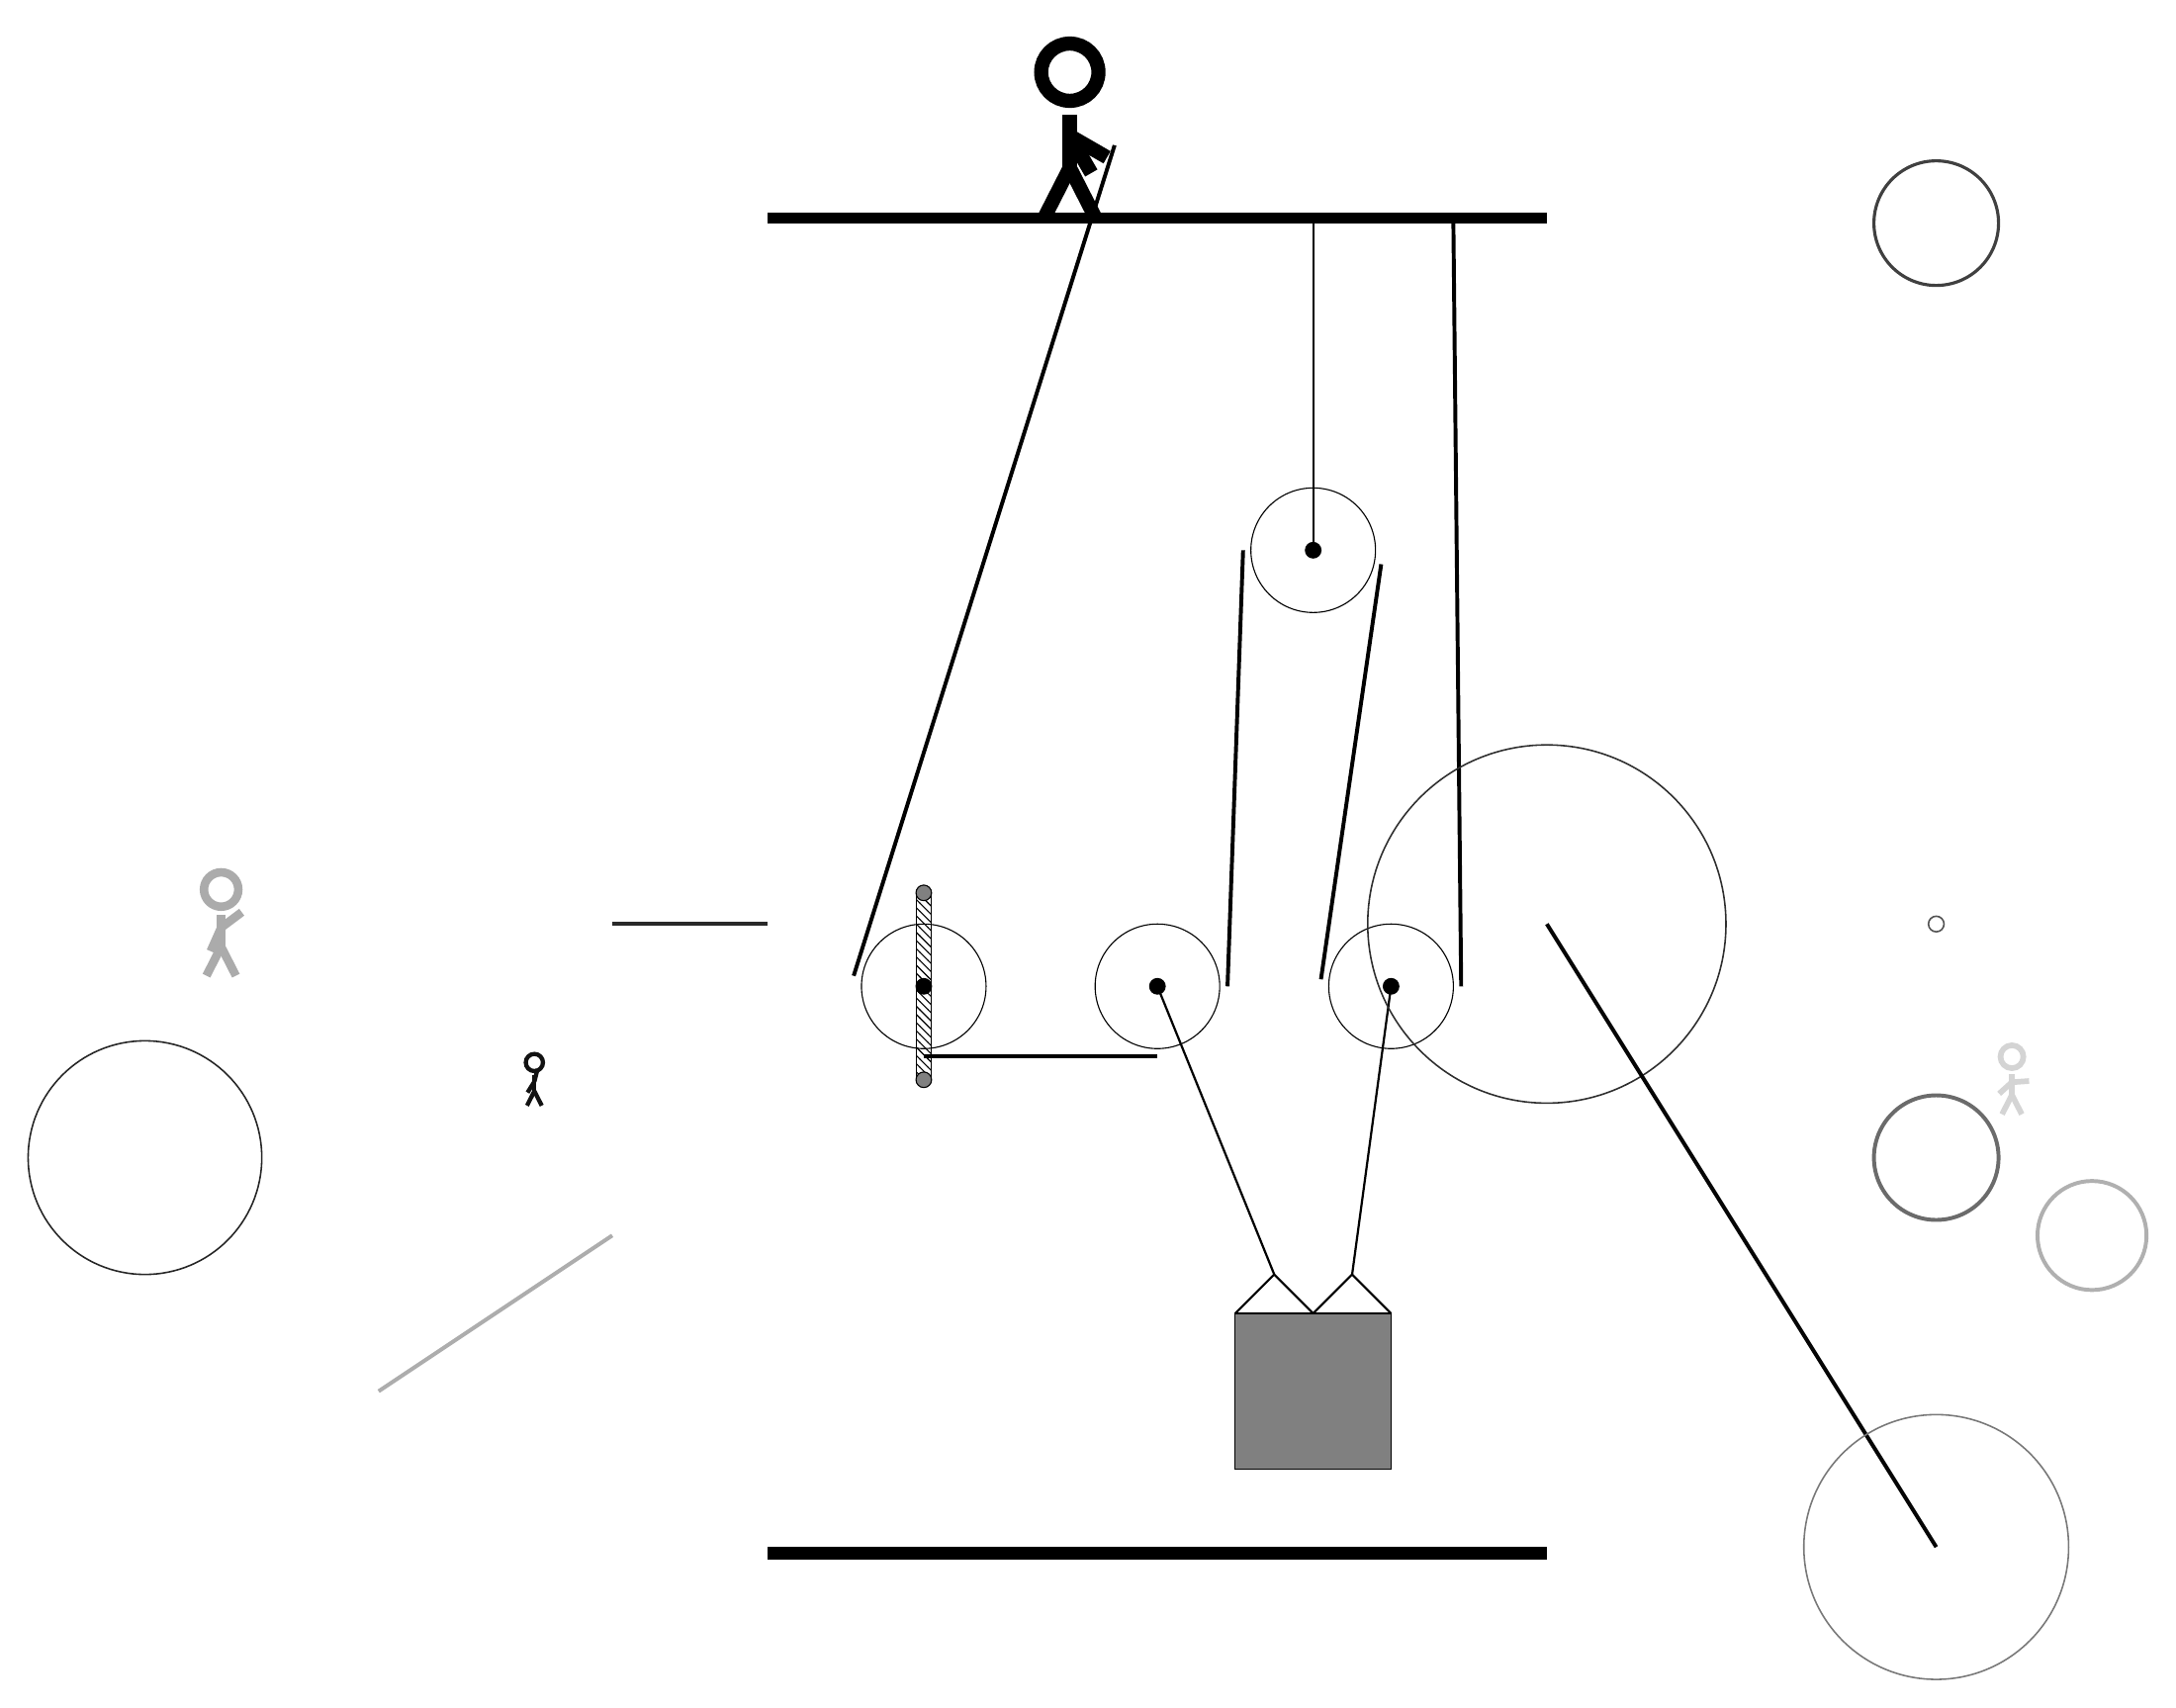
\begin{tikzpicture}
			%%%%% START %%%%%
			
			\draw[fill=black] (-4, 14) rectangle (6, 14.125);
			
			\draw (1, 4.2) circle (0.8);
			\draw[fill=black] (1, 4.2) circle (0.1);
			
			\draw (3, 9.8) circle (0.8);
			\draw[fill=black] (3, 9.8) circle (0.1);
			\draw[thick] (3, 9.8) -- (3, 14);
			
			\draw (4, 4.2) circle (0.8);
			\draw[fill=black] (4, 4.2) circle (0.1);
			
			\draw[thick] (4, 4.2) -- (3.5, 0.5);
			\draw[thick] (1, 4.2) -- (2.5, 0.5);
			\draw[thick]  (2, 0) -- (2.5, 0.5) -- (3, 0);
			\draw[thick]  (3, 0) -- (3.5, 0.5) -- (4, 0);
			\draw[fill=black!50] (2, 0) rectangle (4, -2);
			
			\draw (-2, 4.2) circle (0.8);
			\draw[fill=black] (-2, 4.2) circle (0.1);
			\draw[pattern=north west lines, pattern color=black] (-2.1, 5.4) rectangle (-1.9, 3.0);
			\draw[fill=black!50] (-2, 5.4) circle (0.1);
			\draw[fill=black!50] (-2, 3.0) circle (0.1);
			
			\draw[line width=0.5mm] (0.45, 15) -- (-2.9, 4.335);
			\centerarc[line width=0.5mm](-2, 4.2)(160:270:0.9);
			\draw[line width=0.5mm](-2, 3.3) -- (1, 3.3);
			\centerarc[line width=0.5mm](1, 4.2)(270:360:0.9);
			\draw[line width=0.5mm] (1.9, 4.2) -- (2.1, 9.8);
			\centerarc[line width=0.5mm](3, 9.8)(-20:180:0.9);
			\draw[line width=0.5mm](3.873, 9.62) -- (3.1, 4.29);
			\centerarc[line width=0.5mm](4, 4.2)(160:360:0.9);
			\draw[line width=0.5mm](4.9, 4.2) -- (4.8, 14);
			
			\node[line width=0.6mm, color=black!93] at (-7, 3) {\Strichmaxerl[3][58][76]};
			
			\draw [line width=0.2mm, color=black!82](6, 5) circle (2.3);
			\draw [line width=0.2mm, color=black!68](11, 5) circle (0.1);
			\draw[line width=0.5mm, color=black!98](6, 5) -- (11, -3);
			
			\draw [line width=0.4mm, color=black!75](11, 14) circle (0.8);
			\draw[line width=0.5mm, color=black!32](-6, 1) -- (-9, -1);
			
			\draw [line width=0.2mm, color=black!53](11, -3) circle (1.7);
			
			\draw [line width=0.5mm, color=black!31](13, 1) circle (0.7);
			\node[line width=0.4mm, color=black!33] at (-11, 5) {\Strichmaxerl[6][66][37]};
			
			\draw [line width=0.5mm, color=black!58](11, 2) circle (0.8);
			\draw[line width=0.5mm, color=black!84](-6, 5) -- (-4, 5);
			
			\draw [line width=0.2mm, color=black!85](-12, 2) circle (1.5);
			\node[line width=0.2mm, color=black!17] at (12, 3) {\Strichmaxerl[4][42][4]};
			
			
			\node at (-0.07, 15.2) {\Strichmaxerl[10][120][-30]};
			
			\draw[fill=black] (-4, -3) rectangle (6, -3.15);
			
			%%%%% END %%%%%
		\end{tikzpicture}
	\end{figure}	
\end{document}